




%--------------------------------------------------------%
[fragile]
	{Using \texttt{R} to compute mean (and median)}
When implementing this in R, we would use the following code

\begin{verbatim}
> x1=c(96, 48, 27, 72, 39, 70, 7, 68, 99 )
> sort(x1)
[1]  7 27 39 48 68 70 72 96 99
> median(x1)
[1] 68
>
> x2=c(96, 48 ,27 ,72, 39, 70, 7, 68)
> sort(x2)
[1]  7 27 39 48 68 70 72 96
> median(x2)
[1] 58
\end{verbatim}


%--------------------------------------------------------%
{
	{Dispersion }

\begin{itemize}
\item The data values in a sample are not all the same. This variation between values is called \t{ \emph{dispersion}}.

\item When the dispersion is large, the values are widely scattered; when it is small they are tightly clustered.

%The width of diagrams such as dot plots, box plots, stem and leaf plots is greater for samples with more dispersion and vice versa.

\item
There are several measures of dispersion, the most common being the variance and  standard deviation. These measures indicate to what degree the individual observations of a data set are dispersed or 'spread out' around their mean.

\item
In engineering and science, high precision is associated with low dispersion.
\end{itemize}
}



\chapter{Descriptive Statistics}
Descriptive statistics are used to describe the basic features of the data in a study. They provide simple summaries about the sample and the measures. Together with simple graphics analysis, they form the basis of virtually every quantitative analysis of data.


%===============================================================%

Univariate Analysis

Univariate analysis involves the examination across cases of one variable at a time. There are three major characteristics of a single variable that we tend to look at:

the distribution
the central tendency
the dispersion
In most situations, we would describe all three of these characteristics for each of the variables in our study.


%===============================================================%


The Distribution. The distribution is a summary of the frequency of individual values or ranges of values for a variable. The simplest distribution would list every value of a variable and the number of persons who had each value. For instance, a typical way to describe the distribution of college students is by year in college, listing the number or percent of students at each of the four years. Or, we describe gender by listing the number or percent of males and females. In these cases, the variable has few enough values that we can list each one and summarize how many sample cases had the value. But what do we do for a variable like income or GPA? With these variables there can be a large number of possible values, with relatively few people having each one. In this case, we group the raw scores into categories according to ranges of values. For instance, we might look at GPA according to the letter grade ranges. Or, we might group income into four or five ranges of income values.


%===============================================================%

The Geometric Mean

The Geometric mean is a specialized measure used to calculate the average proportional changes.

Geometric mean formula

$G = \sqrt[n]{(1+p_1) \times (1+p_1) +  \ldots + (1+p_n)}$

The price of a commodity changes by the following percentages over a period of four years.
Compute the average price change.


%%--https://www.mathsisfun.com/data/random-variables.html

%-------------------------------
How to find the $n-th$ root using your calculator.

What is the n-th root of the number $X$

$\sqrt[n]{X} \;= \; X^{1 \over n} $

for example

$\sqrt[5]{11} \;= \; 11^{1 \over 5} \;= \; 11^{0.2} $



%---------------------------
Year 1 Year 2 Year 3 Year 4
Change 10% 5% -8% 12%


The four terms we are going to multiply are
1.10 , 1.05 0.92 and 1.12.


% 1.190112^{0.25}
% 1.044472





%--------------------

\section{Numerical Summaries}
\subsection{Numerical Summaries}
\begin{frame}{\bf \tcb{Numerical Summaries}}
We focus here on \emph{numerical data} only. We have seen how the frequency table and corresponding histogram describe the whole distribution of data.\\[0.4cm]
Often however, we would like to summarise the {\bf main features} of the distribution without using the whole frequency table, i.e., a few numbers - \emph{``numerical summaries''} - which provide the relevant info.\\[0.5cm]
We will look at measures of:
\begin{itemize}\itemsep0.4cm
\item {\bf Centrality} - a numeric value indicating the centre of the distribution, i.e., an ``average'' or ``typical'' value.
\item {\bf Dispersion} - a numeric value indicating the degree to which measurements \emph{vary} about this centre, i.e., is the distribution of values tightly packed around its centre or not?
\end{itemize}

\end{frame}

\subsection{Numerical Summaries}
\begin{frame}{\bf \tcb{Numerical Summaries}\\[-1cm]}
\begin{itemize}\itemsep0.3cm
\item {\bf Centrality}
\begin{itemize}\itemsep0.2cm
\item mean: arithmetic average (you all know this).
\item median: middle number in the \emph{ordered} data.
\end{itemize}
\item {\bf Dispersion}
\begin{itemize}\itemsep0.2cm
\item range: $\max(x) -\min(x)$.
\item variance: measure of variation around the \emph{mean}.
\item standard deviation: square root of the variance.
\item quartiles: \emph{three} numbers - $Q_1$,$Q_2$ and $Q_3$ - which split the \emph{ordered}\newline\phantom{quartiles:} data into four parts (note: $Q_2 =$ the median).
\item inter-quartile range: $IQR = Q_3 - Q_1$.\\[0.4cm]
\end{itemize}
\end{itemize}
We also introduce the {\bf boxplot} - a graphical method for numerical data. This could have gone into the ``Visualising Numerical Data'' section of Lecture 1 but we need $Q_1$,$Q_2$, $Q_3$ and $IQR$ to draw it.
\end{frame}


\section{Centrality}
\subsection{The Mean}
\begin{frame}{\bf \tcb{The Mean}}
The mean is just the usual arithmetic average: add all of the individual data values in the sample and divide by the number of values.\\[0.5cm]
Remember that {\boldmath$n$} is the symbol for the \emph{sample size}, i.e., the number of values. The sample mean is:\\[-0.6cm]

\begin{align*}
\boxed{\bar x = \frac{x_1 + x_2 + \ldots + x_n}{n} = \frac{\sum x_i}{n}}.
\end{align*}

We have introduced the \emph{sum notation} - don't be put off by this! $\sum$ just means ``the sum of'' and $x_i$ means ``individual value''. So $\sum x_i$ means ``the sum of all values''.\\[0.4cm]
Remember that we have seen the symbol $\bar x$ before. Also, recall that it is a \emph{statistic} which \emph{estimates} the population mean $\mu$ \emph{(parameter)}.

\end{frame}

\subsection{The Mean: Example}
\begin{frame}{\bf \tcb{The Mean: Example}}
Let's say we have the annual income (in thousands) of $n = 5$ individuals living in a particular apartment block:
\begin{center}
\begin{tabular}{|ccccc|}
\hline
&&&&\\[-0.4cm]
25 & 29 & 33 & 35 & 40 \\
\hline
\multicolumn{5}{c}{}\\
\end{tabular}
\end{center}
The average income is
\begin{align*}
\bar x = \frac{25 + 29 + 33 + 35 + 40}{5} &= \frac{162}{5} \\[0.2cm]
&= 32.4 \\[0.2cm]
&= \text{\texteuro\,} 32,400.
\end{align*}


\end{frame}



\subsection{The Mean - Skewed Data}
\begin{frame}{\bf \tcb{The Mean - Skewed Data}}
An issue with the mean is its sensitivity to \emph{outliers} - data values much larger / smaller than the main body of data - which lead to \emph{skewness} (remember: data can be skewed to the right / left).\\[0.4cm]
Let's now assume that the 5th individual is \emph{much} wealthier than the others:
\begin{center}
\begin{tabular}{|ccccc|}
\hline
&&&&\\[-0.4cm]
25 & 29 & 33 & 35 & 500 \\
\hline
\multicolumn{5}{c}{}\\
\end{tabular}
\end{center}
The average income is
\begin{align*}
\bar x = \frac{25 + 29 + 33 + 35 + 500}{5} &= \frac{622}{5} \\[0.2cm]
&= 124.4 \\[0.2cm]
&= \text{\texteuro\,} 124,400.
\end{align*}


\end{frame}


\subsection{The Mean - Skewed Data}
\begin{frame}{\bf \tcb{The Mean - Skewed Data}}

It is clear that \texteuro\,124,400 is not a good representation of the centre of the income distribution. It is not a typical income for an individual living in that apartment block.\\[0.6cm]

The mean gets \emph{pulled towards} the outliers, i.e., it is pulled away from the centre in the direction of the skew.\\[0.3cm]
\begin{itemize}\itemsep0.5cm
\item Data skewed to the right (caused by large values) \newline\phantom{\quad}$\Rightarrow$ the mean gets pulled towards the right.\\[0.4cm]
\item Data skewed to the left (caused by small values) \newline\phantom{\quad}$\Rightarrow$ the mean gets pulled towards the left.
\end{itemize}

\end{frame}




\subsection{The Median}
\begin{frame}{\bf \tcb{The Median}}
The median, $Q_2$, is the value that splits the \emph{ordered} data in half:\\
50\% of the data lies above $Q_2$ and 50\% of the data lies below it.\\
{\footnotesize(Note: we call the median $Q_2$ as it is the second quartile - more on this later)}\\[0.6cm]

To find $Q_2$:\\[0.2cm]
\begin{enumerate}[1.]\itemsep0.4cm
\item Put the data \emph{in order} - smallest to largest - if it is not already.
\item $Q_2$ is then the value in \emph{position} $\boxed{\frac{n+1}{2}}$ where $n$ is the sample size.\\[0.6cm]
\end{enumerate}

{\bf Important}: $\tfrac{n+1}{2}$ is not the value of the median, it is its \emph{position} in the\newline\phantom{{\bf Important}:} ordered data.

\end{frame}


\subsection{The Median: Example}
\begin{frame}{\bf \tcb{The Median: Example}\\[-1.1cm]}
\begin{adjustwidth}{-1.5cm}{}
\begin{center}
\begin{tabular}{r|ccccc|}
\multicolumn{1}{c}{} & \multicolumn{5}{c}{\emph{Position}} \\
\multicolumn{1}{c}{} & \emph{1}  & \emph{2}  & \emph{\tcr{3}}  & \emph{4}  & \multicolumn{1}{c}{\emph{5}} \\
\cline{2-6}
&&&&&\\[-0.4cm]
{\bf Symmetrical}: & 25 & 29 & \tcb{33} & 35 & 40 \\
\cline{2-6}
\multicolumn{6}{c}{}\\
\cline{2-6}
&&&&&\\[-0.4cm]
{\bf Skewed to the Right}: & 25 & 29 & \tcb{33} & 35 & 500 \\
\cline{2-6}
\multicolumn{6}{c}{}\\[0.4cm]
\end{tabular}
\end{center}
\end{adjustwidth}
The \emph{\tcr{position}} of the median is:
\begin{align*}
\frac{n+1}{2} = \frac{5+1}{2} = \frac{6}{2} = \tcr{3},\\[-0.6cm]
\end{align*}
i.e., the \tcr{3rd} number.\\[0.4cm]

$\Rightarrow$ The \emph{\tcb{value}} is:\,\, $Q_2 = \tcb{33} = \text{\texteuro}\,33,000$.\\[0.4cm]

The median is unaffected by skewness - it still gives an accurate estimate of the centre.

\end{frame}


\subsection{Mean Vs Median}
\begin{frame}{\bf \tcb{Mean Vs Median}\\[-1.3cm]}
\begin{columns}

\begin{column}{.5\textwidth}
\begin{adjustwidth}{-0.1cm}{0.0cm}
\begin{itemize}\itemsep2.3cm
\item Symmetrical data: $\tcr{\bar x} \approx \tcRg{Q_2}$.
\item Right-skewed: $\tcr{\bar x} > \tcRg{Q_2}$.
\item Left-skewed: $\tcr{\bar x} < \tcRg{Q_2}$.
\end{itemize}
\end{adjustwidth}
\end{column}

\begin{column}{.5\textwidth}
\begin{adjustwidth}{-0.3cm}{0.0cm}

\begin{tabular}{c}
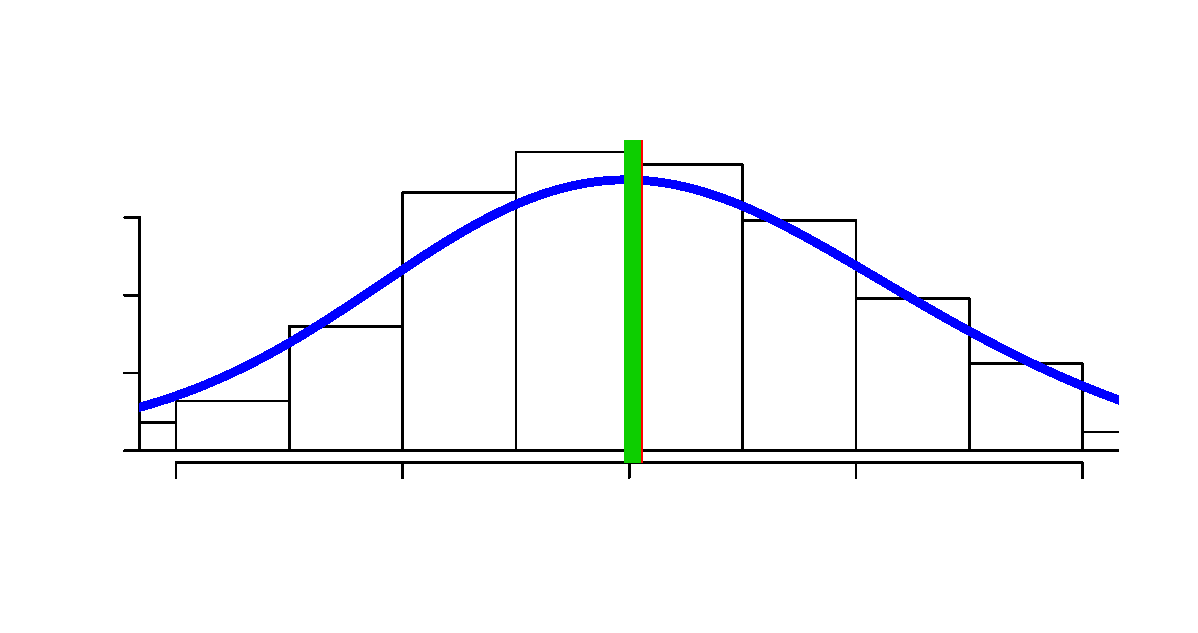
\includegraphics[width=1\textwidth, trim = 0.0cm 0.5cm 0.3cm 1.5cm, clip]{Symmetrical2}\\
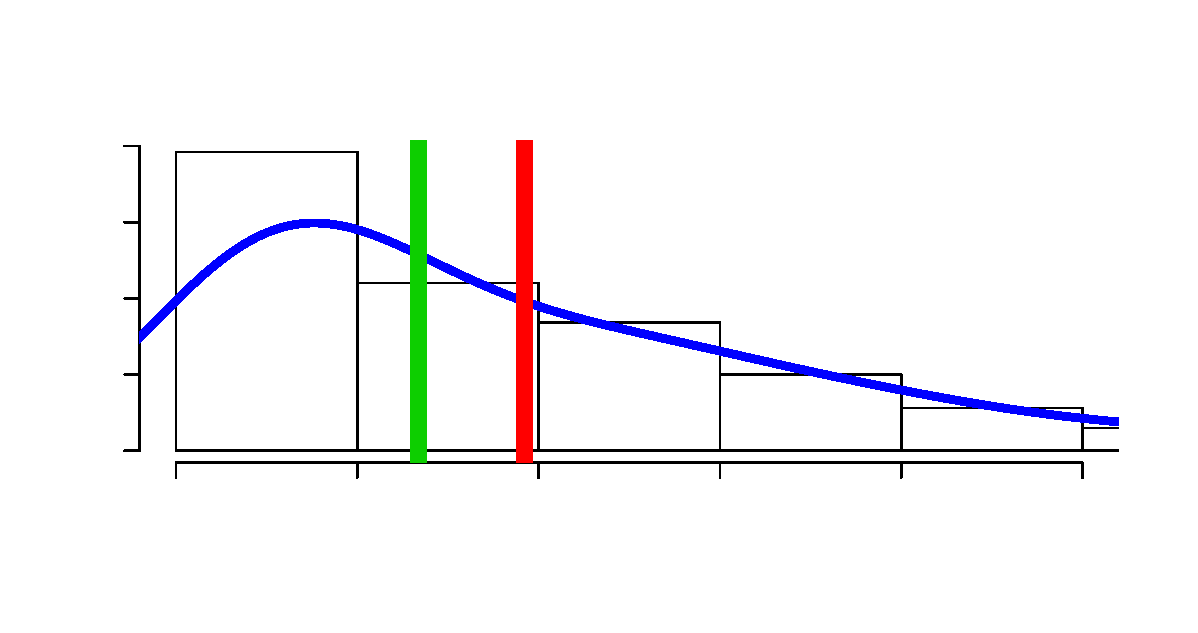
\includegraphics[width=1\textwidth, trim = 0.0cm 0.5cm 0.3cm 1.5cm, clip]{SkewRight2}\\
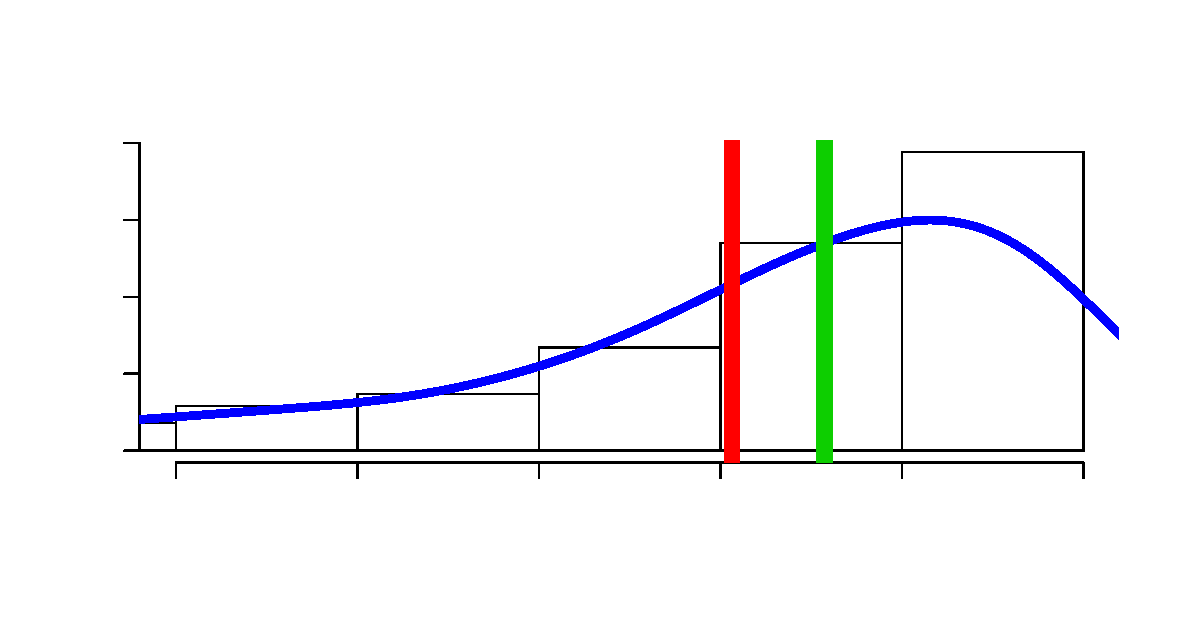
\includegraphics[width=1\textwidth, trim = 0.0cm 0.5cm 0.3cm 1.5cm, clip]{SkewLeft2}
\end{tabular}


\end{adjustwidth}
\end{column}

\end{columns}

\end{frame}


\subsection{The Median: There's No Middle of 6 Numbers!}
\begin{frame}{\bf \tcb{The Median: There's No Middle of 6 Numbers!}}

Let's say we have 6 numbers - what is the median?

\begin{center}
\begin{tabular}{|cccccc|}
\multicolumn{6}{c}{\emph{Position}} \\
\multicolumn{1}{c}{\emph{1}} & \emph{2}  & \emph{\tcr{3}}  & \emph{\tcr{4}}  & \emph{5}  & \multicolumn{1}{c}{\emph{6}} \\
\hline
&&&&&\\[-0.4cm]
10 & 13 & 15 & 21 & 32 & 42 \\
\hline
\multicolumn{6}{c}{}\\[-0.3cm]
\end{tabular}
\end{center}
The \emph{\tcr{position}} of the median is:
\begin{align*}
\frac{n+1}{2} = \frac{6+1}{2} = \frac{7}{2} = \tcr{3.5},\\[-0.6cm]
\end{align*}
i.e., the median lies \emph{between} the \tcr{3rd} and \tcr{4th} numbers.\\[0.5cm]

$\Rightarrow$ Its \emph{\tcb{value}} is simply the \emph{average} of the numbers in position \tcr{3} and \tcr{4}:
\begin{equation*}
Q_2 = \tfrac{15+21}{2} = \tfrac{36}{2} = \tcb{18}.
\end{equation*}

\end{frame}



\subsection{The Standard Deviation - Skewed Data}
\begin{frame}{\bf \tcb{The Standard Deviation - Skewed Data}}

Recall that $\bar x$ is \emph{not} a good measure of centrality when data is skewed (use the median, $Q_2$, instead).\\[0.6cm]
If this is the case, we are then not interested in $s$\, either since this measures the dispersion about $\bar x$.\\[1cm]
So what goes with the median? - The \emph{inter-quartile range}.


\end{frame}


\subsection{Quartiles}
\begin{frame}{\bf \tcb{Quartiles}}

There are {\bf three quartiles} which split the (ordered!) data into four parts:\\[-0.4cm]
\begin{align*}
25\% - {\bf Q_1} - 25\% - {\bf Q_2} - 25\% - {\bf Q_3} - 25\%
\end{align*}
The process of finding the quartiles is essentially the same as the case of finding the median (i.e., the second quartile $Q_2$).\\[0.4cm]
\begin{enumerate}[1.]
\item Put the data \emph{in order} - smallest to largest.
\item The \emph{position} of $Q_k$ (quartile number $k$) is:
    \boxed{\frac{n+1}{4}\times k}.\\[0.6cm]
\end{enumerate}

$Q_1$ is in position $\tfrac{n+1}{4}$, $Q_2$ is in position $\tfrac{n+1}{4}\times2$ and $Q_3$ is in position $\tfrac{n+1}{4}\times3$.

\end{frame}


\subsection{The Inter-Quartile Range}
\begin{frame}{\bf \tcb{Inter-Quartile Range}}

The {\bf inter-quartile range} is the range of the middle 50\% of data.\\[1.2cm]

Calculation of IQR is straightforward once we have the quartiles:
\begin{align*}
\boxed{IQR = Q_3 - Q_1},\\[-0.1cm]
\end{align*}
i.e., it is simply the difference between the upper and lower quartiles.

\end{frame}




\subsection{Quartiles and IQR: Example}
\begin{frame}{\bf \tcb{Quartiles and IQR: Example}}
Consider the following sample of $n=10$ values:\\[-0.2cm]
\begin{center}
\begin{tabular}{|cccccccccc|}
\hline
&&&&&&&&&\\[-0.4cm]
2 & 4 & 2 & 1 & 5 & 3 & 0 & 4 & 1 & 8 \\
\hline
\end{tabular}
\end{center}
First we must \emph{sort} the values. The reordered dataset is:\\[-0.2cm]
\begin{center}
\begin{tabular}{|ccccccccccc|}
\multicolumn{1}{c}{\emph{Positions:}} & \multicolumn{1}{c}{\emph{1}} & \emph{\tcr{2}} & \emph{\tcr{3}} & \emph{4} & \emph{\tcb{5}} & \emph{\tcb{6}} & \emph{7} & \emph{\tcRg{8}} & \emph{\tcRg{9}} & \multicolumn{1}{c}{\emph{10}} \\
\cline{1-11}
&&&&&&&&&&\\[-0.4cm]
\multicolumn{1}{|c}{\emph{Values:}} & 0 & 1 & 1 & 2 & 2 & 3 & 4 & 4 & 5 & 8 \\
\cline{1-11}
\end{tabular}
\end{center}


\begin{tabular}{c|c|c}
{\bf Quartile} & {\bf Position} & {\bf Value} \\[0.1cm]
$Q_1$ & $\tfrac{10+1}{4} = \tfrac{11}{4} = 2.75$\,\,$\Rightarrow$ between \tcr{2} \& \tcr{3} & $\tfrac{1+1}{2} = {\bf1}$\\[0.3cm]
$Q_2$ & $\tfrac{11}{4}\times2 = 2.75\times2 = 5.5$\,\,$\Rightarrow$ between \tcb{5} \& \tcb{6} & $\tfrac{2+3}{2} = {\bf2.5}$\\[0.3cm]
$Q_3$ & $\tfrac{11}{4}\times3 = 2.75\times3 = 8.25$ $\Rightarrow$ between \tcRg{8} \& \tcRg{9} & $\tfrac{4+5}{2} = {\bf4.5}$\\
\multicolumn{3}{c}{}\\
\end{tabular}

$\Rightarrow$ {\bf IQR} $= Q_3 - Q_1 = 4.5 - 1 = {\bf3.5}$. \\
{\footnotesize (3.5 units covers the middle 50\% of data)}

\end{frame}


\subsection{Question 3}
\begin{frame}{\bf \tcb{Question 3}}
We return to the laptop battery life data:\\
\begin{center}
\begin{tabular}{|cccccccccc|}
\hline
&&&&&&&&&\\[-0.4cm]
2.2 & 0.4 & 4.2 & 12.9 & 1.5 & 3.0 & 5.7  & 0.7 & 1.0 & 3.3 \\
0.2 & 0.2 & 5.6 &  1.6 & 3.0 & 0.1 & 14.3 & 3.4 & 0.9 & 6.1 \\
1.4 & 1.0 & 0.7 & 5.4  & 2.3 &&&&&\\
\hline
\end{tabular}
\end{center}
\begin{enumerate}[a)]\itemsep0.3cm
\item What is the value of $n$\,?
\item Find the values of the quartiles.
\item Calculate IQR.
\item Calculate $\bar x$ and compare this to $Q_2$. Is the data skewed? If so, in what direction?
\end{enumerate}
\end{frame}




\section{Question 4}
\begin{frame}{\bf \tcb{Question 4}}
It turns out that the laptops can be split into two groups. The battery lives for each of the 25 laptops is shown below:\vspace{-0.2cm}
\begin{adjustwidth}{-0.3cm}{}
\begin{tabular}{|cccccccccccc|}
\hline
&&&&&&&&&&&\\[-0.4cm]
Type 1: & 0.1 & 0.2 & 0.2 & 0.4 & 0.7 & 0.9 & 1.0 & 1.5 & 2.3 & 4.2 & 5.6 \\[0.1cm]
\hline
&&&&&&&&&&&\\[-0.4cm]
Type 2: & 0.7 & 1.0 & 1.4 & 1.6 & 2.2 & 3.0 & 3.0 & 3.3 & 3.4 & 5.4 & 5.7 \\
& 6.1 & 12.9 & 14.3 &&&&&&&&\\
\hline
\end{tabular}
\end{adjustwidth}
\begin{enumerate}[a)]\itemsep0.3cm
\item Calculate the means for the two groups: $\bar x_1$ and $\bar x_2$.
\item What are the values of $n_1$ and $n_2$?
\item Draw the boxplots for each group (side by side on the same graph) and comment.
\item Are there outliers in either group?
\item Are either of the distributions skewed? If so, in what direction?
\end{enumerate}
\end{frame}



\section{Symbols}
\subsection{Recap of Symbols}
\begin{frame}{\bf \tcb{Recap of Symbols}}
Firstly, the sample size is $n$. The other symbols are given below:\\[0.3cm]
\begin{center}
\begin{tabular}{|c|c|c|}
\hline
&&\\[-0.3cm]
& Sample & Population \\
Quantity & Statistic & Parameter \\[0.1cm]
\hline
&&\\[-0.3cm]
Proportion & $\hat p$ & $p$ \\[0.2cm]
Mean & $\bar x$ & $\mu$ \\[0.2cm]
Variance & $s^2$ & $\sigma^2$ \\[0.2cm]
Standard Deviation & $s$\phantom{$^2$} & $\sigma$\phantom{$^2$} \\[0.2cm]
Quartiles & $Q_1$, $Q_2$, $Q_3$ & ---\\[0.2cm]
\hline
\multicolumn{3}{c}{}\\
\end{tabular}
\end{center}
{\footnotesize(we did not assign symbols to population quartiles)}
\end{frame}

%--------------------------------------------------------%

\section{Descriptive Statistics}

%{
%
%	{Descriptive Statistics}
%
%\begin{itemize}
%\item Measures of Centrality
%\begin{itemize}
%\item Mean
%\item Median
%\end{itemize}
%\item Measures of Dispersion
%\begin{itemize}
%\item Range
%\item Variance
%\item Standard Deviation
%\end{itemize}
%% \item Quantiles
%% \item Distribution of data ( Skewed or Symmetric )
%\end{itemize}
%
%}
\section{R Code}
\subsection{R Code: Centrality}
\begin{frame}{\bf \tcb{R Code: Centrality}}
The code used to calculate the mean and median for the income example is:\\[0.6cm]
\begin{tabular}{|l|}
\hline
\texttt{income = c(25, 29, 33, 35, 40)}\\
\texttt{mean(income)}\\
\texttt{median(income)}\\
\hline
\multicolumn{1}{c}{}\\[-0.1cm]
\end{tabular}

\end{frame}

\subsection{R Code: Dispersion}
\begin{frame}{\bf \tcb{R Code: Dispersion}}
The code used to calculate the variance and standard deviation for the income example is:\\[0.1cm]
\begin{tabular}{|l|}
\hline
\texttt{income = c(25, 29, 33, 35, 40)}\\
\texttt{var(income)}\\
\texttt{sd(income)}\\
\hline
\multicolumn{1}{c}{}\\[0.1cm]
\end{tabular}

Quartiles (as well as the minimum, maximum and mean) are given by the \texttt{summary} function:\\[0.1cm]
\begin{tabular}{|l|}
\hline
\texttt{x = c(2, 4, 2, 1, 5, 3, 0, 4, 1, 8)}\\
\texttt{summary(x)}\\
\hline
\multicolumn{1}{c}{}\\[-0.1cm]
\end{tabular}

R uses a slightly different method for calculating $Q_1$ and $Q_3$ to what we use in this course - so the results will be different to the lecture.\\[0.4cm]

Finally IQR is found via $\boxed{\text{\texttt{IQR(x)}}}$ - again different to the lecture.
\end{frame}


\subsection{R Code: Sort}
\begin{frame}{\bf \tcb{R Code: Sort}}
Another useful function is the \texttt{sort} function which orders the data from smallest to largest.\\[0.3cm]

\begin{tabular}{|l|}
\hline
\texttt{laptop = c(2.2, 0.4,  4.2, 12.9,  1.5,}\\
\hspace{2.5cm}\texttt{3.0,  5.7,  0.7,  1.0,  3.3,}\\
\hspace{2.5cm}\texttt{0.2,  0.2,  5.6,  1.6,  3.0,}\\
\hspace{2.5cm}\texttt{0.1, 14.3,  3.4,  0.9,  6.1,}\\
\hspace{2.5cm}\texttt{1.4,  1.0,  0.7,  5.4,  2.3)}\\
\texttt{laptop = sort(laptop)}\\
\texttt{laptop}\\
\hline
\multicolumn{1}{c}{}\\[-0.1cm]
\end{tabular}

\end{frame}



\subsection{R Code: Boxplot}
\begin{frame}{\bf \tcb{R Code: Boxplot}}
Using the \texttt{laptop} data from the previous slide, we can draw a boxplot (and include the mean) using\\[0.3cm]
\begin{tabular}{|l|}
\hline
\texttt{boxplot(laptop, xlab="Battery Life (hours)")}\\
\texttt{points(x=1,y=mean(laptop),pch=20)}\\
\hline
\multicolumn{1}{c}{}\\[-0.3cm]
\end{tabular}

{\footnotesize(Remember that R uses a different formula to get $Q_1$ and $Q_3$. So the boxplot will be slightly different to the one you do by hand)}\\[0.7cm]


A horizontal boxplot is given by\\[0.3cm]
\begin{tabular}{|l|}
\hline
\texttt{boxplot(laptop, horizontal=T, }\\
\hspace{2cm}\texttt{xlab="Battery Life (hours)")}\\
\texttt{points(x=mean(laptop),y=1,pch=20)}\\
\hline
\multicolumn{1}{c}{}\\[-0.1cm]
\end{tabular}
\end{frame}


\subsection{R Code: Two Boxplots}
\begin{frame}{\bf \tcb{R Code: Two Boxplots}}
Two boxplots side by side with mean values shown:\\[0.2cm]
\begin{tabular}{|l|}
\hline
\texttt{laptop1 = c(0.1, 0.2,  0.2, 0.4,  0.7, 0.9,  1.0,}\\
\hspace{2.8cm}\texttt{1.5, 2.3,  4.2, 5.6)}\\
\texttt{laptop2 = c(0.7, 1.0, 1.4, 1.6, 2.2, 3.0, 3.0,}\\
\hspace{2.8cm}\texttt{3.3, 3.4, 5.4, 5.7, 6.1, 12.9, 14.3)}\\[0.2cm]
\texttt{boxplot(laptop1,laptop2,}\\
\hspace{2.8cm}\texttt{xlab="Battery Life (hours)")}\\
\texttt{points(x=1,y=mean(laptop1),pch=20)}\\
\texttt{points(x=2,y=mean(laptop2),pch=20)}\\
\hline
\multicolumn{1}{c}{}\\[-0.1cm]
\end{tabular}


 

\end{frame}

